\section{Materia Prima}

\begin{equation*}
\centering
   Desv. \; Eficiencia + Desv. \; Precio  = Desviacion \; Contable
\end{equation*}

\tikzset{every picture/.style={line width=0.75pt}} %set default line width to 0.75pt        

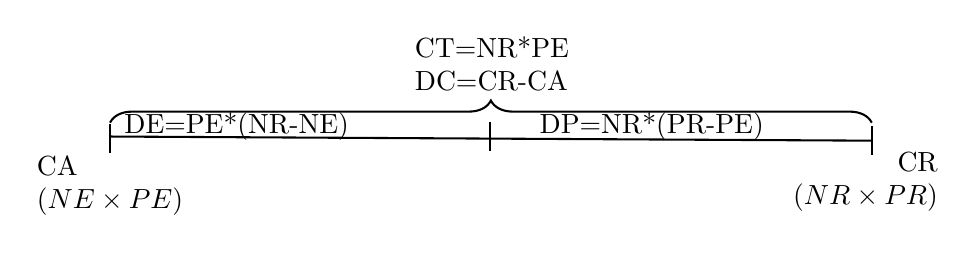
\begin{tikzpicture}[x=0.75pt,y=0.75pt,yscale=-1,xscale=1]
\centering

\draw    (94,110) -- (461,112) ;
\draw    (94,104) -- (94,118) ;
\draw    (277,103) -- (277,117) ;
\draw    (461,105) -- (461,119) ;
\draw[decorate, decoration = {brace, amplitude = 8pt}, xshift = 0pt, yshift = 10pt] (94, 90) -- (461, 90);
\draw (458,132) node  [align=right] {CR \\ ($NR \times PR$)};
\draw (94,134) node  [align=left] {CA \\ ($NE \times PE$)};
\draw (278,75) node  [align=left] {CT=NR*PE \\ DC=CR-CA};
\draw (355,105) node  [align=left] {DP=NR*(PR-PE)};
\draw (155,105) node  [align=left] {DE=PE*(NR-NE)};

\end{tikzpicture}

\section{Mano de Obra}

\begin{equation*}
\centering
   Desv. \; Eficiencia + Desv. \; Tasa \; Salarial  = Desviacion \; Contable
\end{equation*}

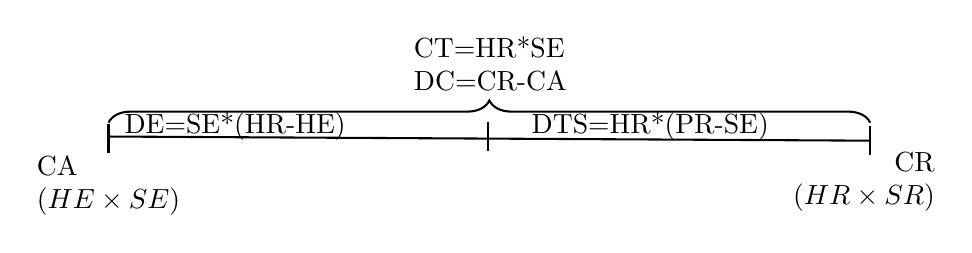
\begin{tikzpicture}[x=0.75pt,y=0.75pt,yscale=-1,xscale=1]
\centering

\draw    (94,110) -- (461,112) ;
\draw    (94,104) -- (94,118) ;
\draw    (277,103) -- (277,117) ;
\draw    (461,105) -- (461,119) ;
\draw[decorate, decoration = {brace, amplitude = 8pt}, xshift = 0pt, yshift = 10pt] (94, 90) -- (461, 90);
\draw (458,132) node  [align=right] {CR \\ ($HR \times SR$)};
\draw (94,134) node  [align=left] {CA \\ ($HE \times SE$)};
\draw (278,75) node  [align=left] {CT=HR*SE \\ DC=CR-CA};
\draw (355,105) node  [align=left] {DTS=HR*(PR-SE)};
\draw (155,105) node  [align=left] {DE=SE*(HR-HE)};

\end{tikzpicture}
